\documentclass[]{beamer}

\usepackage{tikz}
\usepackage{xspace}

\newcommand{\States}{\ensuremath{T}\xspace}		% Set of States
\newcommand{\state}{\ensuremath{t}\xspace}		% single states
\newcommand{\mystate}[1]{\ensuremath{\state_{\mathrm{#1}}}\xspace} %meaningful states
\newcommand{\Messgs}{\ensuremath{M}\xspace}		% Set of Messages
\newcommand{\messg}{\ensuremath{m}\xspace}		% single messages
\newcommand{\mymessg}[1]{\ensuremath{\messg_{\mathrm{#1}}}\xspace} %meaningful messages
\newcommand{\cost}{\ensuremath\mathrm{C}} % cost function
\newcommand{\Acts}{\ensuremath{A}\xspace}		% Set of R-actions
\newcommand{\act}{\ensuremath{a}\xspace}		% single action
\newcommand{\myact}[1]{\ensuremath{\act_{\mathrm{#1}}}\xspace} %meaningful

\begin{document}


\begin{frame}
  \frametitle{Lewis games (type matching)}
    \begin{center}
      \vspace{-0.35cm}
      \begin{tikzpicture}[rounded corners]

        \node at (0,0)
        {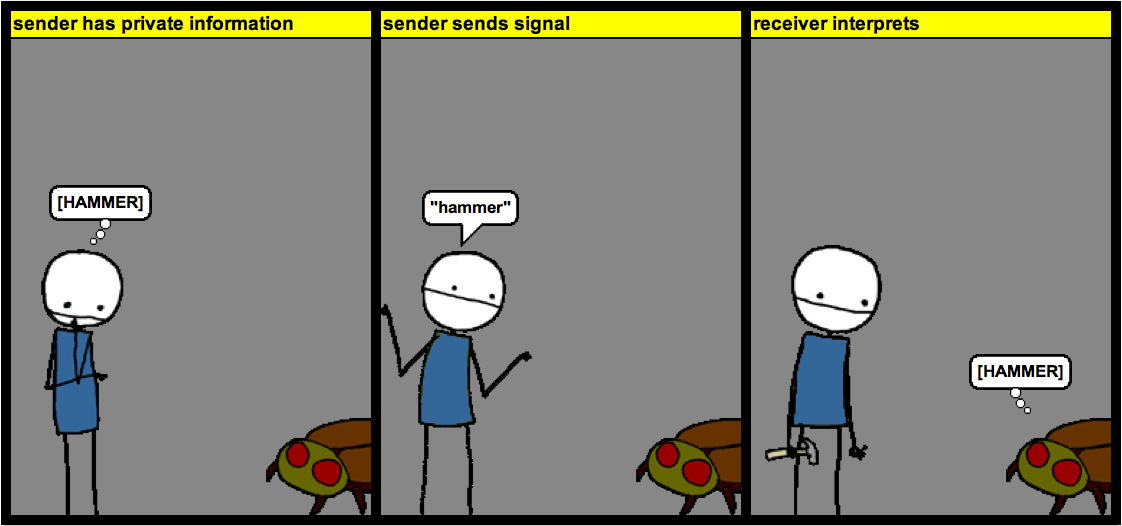
\includegraphics[width=10cm]{Comic_SG_success.png}};

        \node at (-3.5,-2.7) {$\mystate{s} \in \States$};

        \node at (0,-2.7) {$\messg \in \Messgs$};

        \node at (3.5,-2.7) {$\mystate{r} \in \States$};

        \node[text width = 2.8cm, text centered, draw=green!50,
        fill=green!20, thick] at (3.5,-4) {$\mystate{s} =
          \mystate{r}$ \\ $\Updownarrow$ \\  {success}};

      \end{tikzpicture}
    \end{center}

\end{frame}

\begin{frame}
  \frametitle{Lewis games (type matching)}
    \begin{center}
      \vspace{-0.35cm}
      \begin{tikzpicture}[rounded corners]

        \node at (0,0)
        {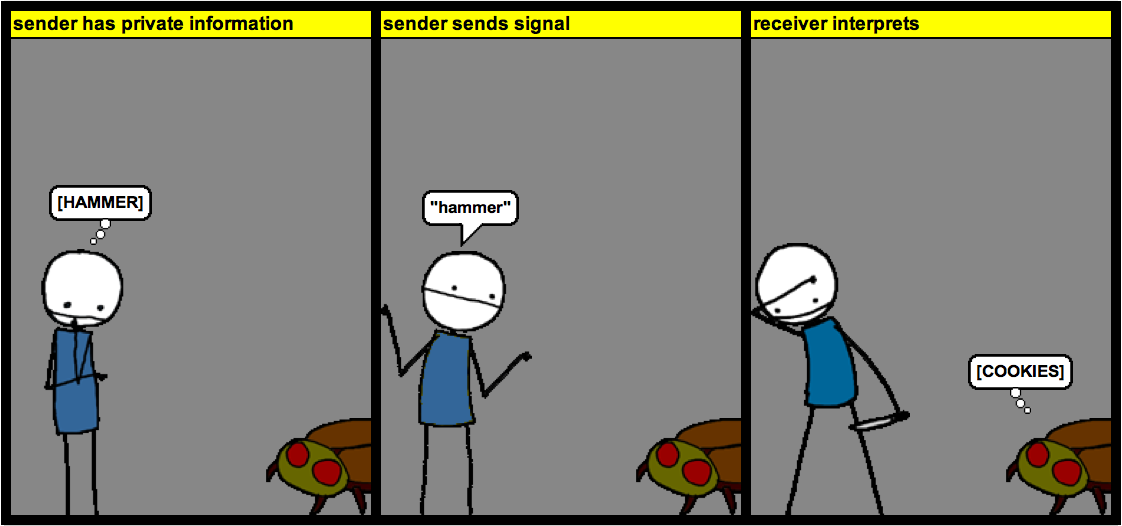
\includegraphics[width=10cm]{Comic_SG_failure.png}};

        \node at (-3.5,-2.7) {$\mystate{s} \in \States$};

        \node at (0,-2.7) {$\messg \in \Messgs$};

        \node at (3.5,-2.7) {$\mystate{r} \in \States$};

        \node[text width = 2.8cm, text centered, draw=red!50,
        fill=red!20, thick] at (3.5,-4) {$\mystate{s} \neq
          \mystate{r}$ \\ $\Updownarrow$ \\  {failure}};

      \end{tikzpicture}
    \end{center}

\end{frame}

\begin{frame}
  \frametitle{Similarity maximizing games}

    \begin{center}
      \vspace{-0.35cm}
      \begin{tikzpicture}[rounded corners]

        \node at (0,0)
        {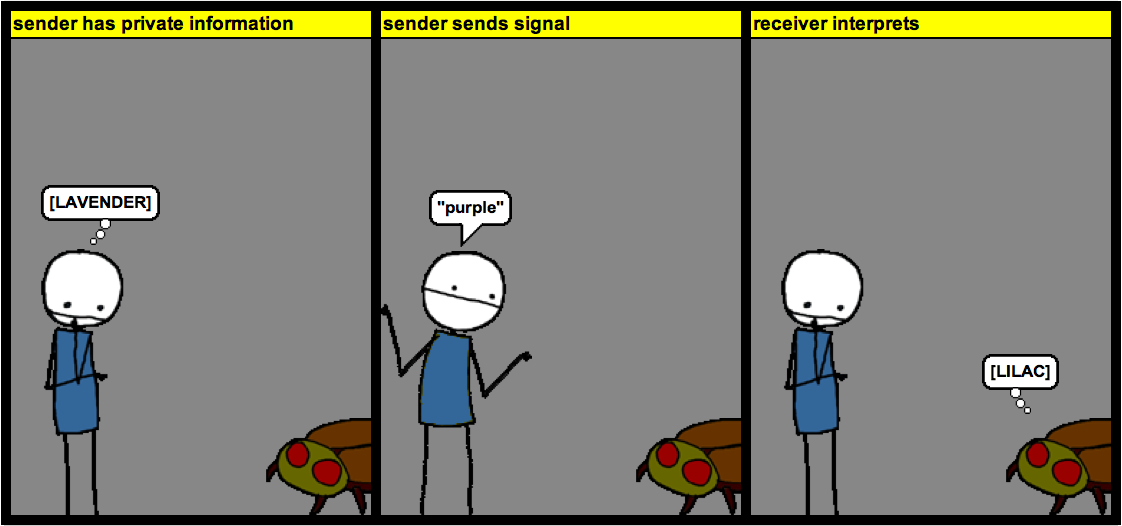
\includegraphics[width=10cm]{Comic_SG_partial_success.png}};

        \node at (-3.5,-2.7) {$\mystate{s} \in \States$};

        \node at (0,-2.7) {$\messg \in \Messgs$};

        \node at (3.5,-2.7) {$\mystate{r} \in \States$};

        \node[text width = 2.8cm, text centered, draw=blue!50,
        fill=blue!20, thick] at
        (3.5,-4) {success \\ $\propto$ \\ $\mathtt{similarity}(\mystate{s},\mystate{r})$};

      \end{tikzpicture}
    \end{center}

     
\end{frame}

\begin{frame}
  \frametitle{Similarity maximizing games}
  \framesubtitle{Example}

    \begin{center}
      \vspace{-0.35cm}

      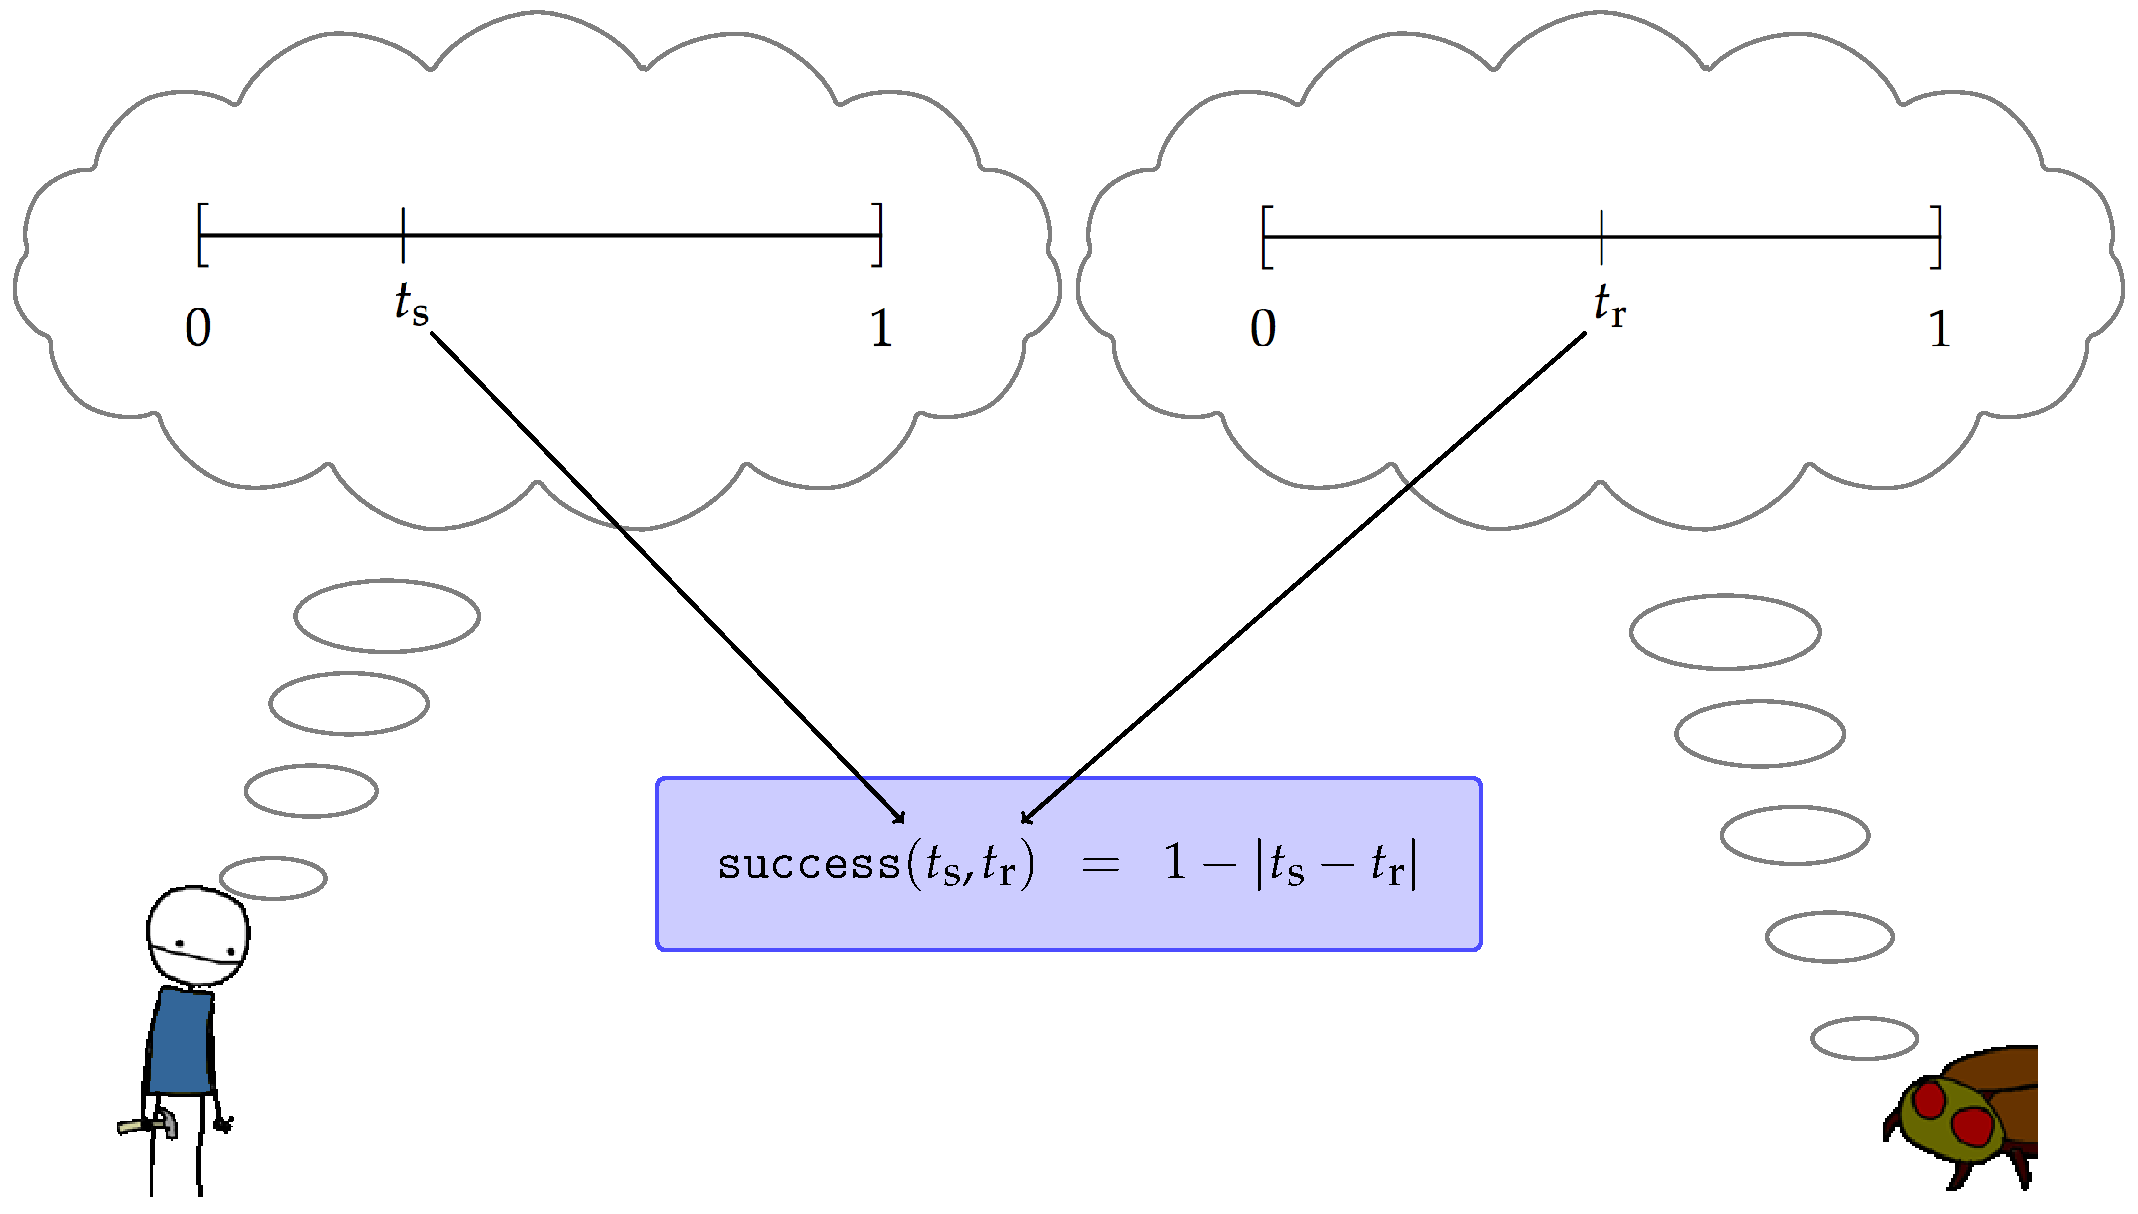
\includegraphics[width=\textwidth]{Comic_sim_max.pdf}

     \end{center}

\end{frame}





\end{document}
